\documentclass[main.tex]{subfiles}
\begin{document}

\chapter{Algoritmes}
\label{cha:algoritmes}

\section{Jordanmatrix berekenen}

\subsection*{Abstract}

\subsubsection*{Vraag}
Gegeven is de lineaire afbeelding $\mathcal{A}:\ \mathbb{C}^{n} \rightarrow \mathbb{C}^{n}$ met $A$ als matrix ten opzichte van de standaarbasis van $\mathbb{C}$.
Bepaal de jordanvorm $J$ van $A$ en geef de $P$ zodat $J=P^{-1}AP$ geldt.
Geef ook de karakteristieke veelterm en de minimale veelterm van $A$.
\subsubsection*{Antwoord}
\begin{itemize}
\item Bereken de karakteristieke veelterm van $A$.
  \[ f_{A}(X) = \prod_{i=1}^{q}(X-c_{i})^{n_{i}} \]
\item Componenten van de vectorruimten bepalen:
  \[ V_{i} = Ker(A-c_{i}I)^{p_{i}} \]
  We bepalen de $p_{i}$ als volgt:
  Bepaal de dimensie van $A-c_{i}I$, $(A-c_{i}I)^{2}$,...
  \[ dim(Ker(A-c_{i}I)^{j}) = n-dim((A-c_{i}I)^{j}) \]
  Ga door met $j$ te verhogen tot $dim(Ker(A-c_{i}I)^{j})$ $dim(V_{i})$ is.
  $p_{i}$ is dan $j$.
\item Diagram voor elke $V_{i}$
  Definieer nu $d_{i}$ als volgt:
  \[ d_{1} = dim(Ker(A-c_{i}I)) \text{ en } d_{j} = dim(Ker(A-c_{i}I)^{j}-dim(Ker(A-c_{i}I)^{j-1} \]
  Maak voor elke $V_{i}$ een diagram van rijen `doosjes' met op de $j$-de rij $d_{j}$ doosjes.
  Vul dan het diagram in als volgt: (begin onderaan links)
  \begin{itemize}
  \item Vul de dozen in rij $k$ op met lineair onafhankelijke vectoren uit $Ker(A-c_{i}I)^{k}\setminus Ker(A-c_{i}I)^{k-1}$.
  \item Vul de doos boven een gevulde doos met vector $v$ op met de vector $(A-c_{i}I)v$.
  \item Als de huidige doos de onderste uit een rij is, vul deze dan in met een vector die onafhankelijk is van de vectoren links ervan.
  \end{itemize}
\item Maak een matrix $P$ door de collecties vectoren als de kolommen in een matrix te zetten.
\item Maak de Jordanmatrix door de eigenwaarden op de diagonaal de zetten, en een $1$ er links van als de overeenkomstige vector in een doos zit waar nog een vector onder staat.
\end{itemize}

\subsection*{Voorbeeld}

\subsubsection*{Vraag}
Gegeven is de lineaire afbeelding $\mathcal{A}:\ \mathbb{C}^{5} \rightarrow \mathbb{C}^{5}$ met $A$ als matrix ten opzichte van de standaarbasis van $\mathbb{C}$.
\[
\begin{pmatrix}
  1 & 1 & -2 & -3 & 0\\
  0 & 3 & 0 & -2 & 0\\
  0 & -1 & 3 & 3 & 0\\
  0 & 0 & 0 & 1 & 0\\
  -1 & 2 & -1 & -2 & 1
\end{pmatrix}
\]
Bepaal de jordanvorm $J$ van $A$ en geef de $P$ zodat $J=P^{-1}AP$ geldt.
Geef ook de karakteristieke veelterm en de minimale veelterm van $A$.
\subsubsection*{Antwoord}
\begin{itemize}
\item 
  \[
  \begin{array}{rll}
    \begin{vmatrix}
      X-1 & -1 & 2 & 3 & 0\\
      0 & X-3 & 0 & 2 & 0\\
      0 & 1 & X-3 & -3 & 0\\
      0 & 0 & 0 & X-1 & 0\\
      1 & -2 & 1 & 2 & X-1
    \end{vmatrix}
    &= 
    (X-1) 
    \begin{vmatrix}
      X-1 & -1 & 2 & 3 \\
      0 & X-3 & 0 & 2 \\
      0 & 1 & X-3 & -3 \\
      0 & 0 & 0 & X-1 
    \end{vmatrix} &\\
    &=
    (X-1)^{2}
    \begin{vmatrix}
      X-1 & -1 & 2 \\
      0 & X-3 & 0\\
      0 & 1 & X-3
    \end{vmatrix} &\\
    &= 
    (X-1)^{3}
    \begin{vmatrix}
      X-3 & 0\\
      1 & X-3
    \end{vmatrix} &\\
    &=
    (X-1)^{3}(X-3)^{2}
  \end{array}
  \]
\item De vectorruimte valt uit elkaar in twee componenten:
  \[ \mathbb{C}^{5} = Ker(A-I)^{p_{1}} \oplus Ker(A-3I )^{p_{2}} \]
  De dimensies zijn als volgt:
  \[ dim(V_{1})= 3 \text{ en } dim(V_{2}) = 2\]
  \begin{itemize}
  \item $V_{1}$
    \begin{itemize}
    \item
      \[ dim(A-I) = dim
      \begin{pmatrix}
        0 & 1 & -2 & -3 & 0\\
        0 & 1 & 0 & -2 & 0\\
        0 & -1 & 2 & 3 & 0\\
        0 & 0 & 0 & 0 & 0\\
        -1 & 2 & -1 & -2 & 0
      \end{pmatrix}
      = 3 \Rightarrow dim(Ker(A-I)) = 2
      \]
    \item
      \[ dim(A-I)^{2} = dim
      \begin{pmatrix}
        0 & 4 & -4 & -8 & 0\\
        0 & 4 & 0 & -4 & 0\\
        0 & -4 & 4 & 0 & 0\\
        0 & 0 & 0 & 0 & 0\\
        0 & 4 & 0 & -4 & 0
      \end{pmatrix}
      = 2 \Rightarrow dim(Ker(A-I)^{2}) = 3 \overset{!}{=} dim(V_{1})
      \Rightarrow p_{1} = 2
      \]
    \end{itemize}
  \item $V_{2}$
    \begin{itemize}
    \item
      \[
      dim(A-3I) = dim
      \begin{pmatrix}
        -2 & 1 & -2 & -3 & 0\\
        0 & 0 & 0  & -2 & 0\\
        0 & -1 & 0 & 3 & 0\\
        0 & 0 & 0 & -2 & 0\\
        -1 & 2 & -1 & -2 & -2
      \end{pmatrix}
      =  4 \Rightarrow dim(Ker(A-3I)) = 1
      \]
    \item 
      \[ 
      dim((A-3I)^{2}) = dim
      \begin{pmatrix}
        4 & 0 & 4 & 4 & 0\\
        0 & 0 & 0 & 4 & 0\\
        0 & 0 & 0 & -4& 0\\
        0 & 0 & 0 & 4 & 0\\
        4 & -4 & 4 & 4 & 4
      \end{pmatrix}
      = 3 \Rightarrow dim(Ker(A-3I)) = 2 \overset{!}{=} dim(V_{2}) \Rightarrow p_{2} = 2
      \]
    \end{itemize}
  \end{itemize}
\item diagram
  \begin{itemize}
  \item $V_{1}$\\
    $d_{1} = 2$ en $d_{2} = 1$, dus het diagram ziet er al volgt uit:
    \[
    \begin{array}{cc}
      \boxed{v_{2}} & \boxed{v_{3}}\\
      \boxed{v_{1}}
    \end{array}
    \] 
    $v_{1}$ moet in $Ker(A-I)^{2}\setminus Ker(A-I)$ zitten.
    Kies bijvoorbeeld $v_{1} = (1,0,0,0,0)$.
    $v_{2}$ staat boven $v_{1}$, dus $v_{2}$ moet $(A-I)v_{1}= (0,0,0,0,-1)$ zijn.
    Kies nu een vector $v_{3}$, lineair onafhankelijk van $v_{2}$, uit $Ker(A-I)$.
    Bijvoorbeeld $v_{3} = (1,1,-1,1,0)$.
    
  \item $V_{2}$\\
    $d_{1} = 1$ en $d_{2} = 1$, dus het diagram ziet er als volgt uit:
    \[
    \begin{array}{c}
      \boxed{v_{2}}\\
      \boxed{v_{1}}
    \end{array}
    \]
    $v_{1}$ moet in $Ker(A-3I)^{2}\setminus Ker(A-3I)$ zitten.
    Kies bijvoorbeeld $v_{1}= (0,1,0,0,1)$.
    $v_{2}$ staat boven $v_{1}$, dus $v_{2}$ moet $(A-3I)v_{1}= (1,0,-1,0,0)$ zijn.

  \end{itemize}
\item 
  \[ P = 
  \left(
    \begin{array}{ccc|cc}
      1 & 0 & 1 & 0 & 1\\
      0 & 0 & 1 & 1 & 0\\
      0 & 0 & -1& 0 &-1\\
      0 & 0 & 1 & 0 & 0\\
      0 & -1& 0 & 1 & 0\\
    \end{array}
  \right)
  \]
\item 
  \[ J =
  \left(
    \begin{array}{ccc|cc}
      1 & 0 & 0 & 0 & 0\\
      1 & 1 & 0 & 0 & 0\\
      0 & 0 & 1 & 0 & 0\\\hline
      0 & 0 & 0 & 3 & 0\\
      0 & 0 & 0 & 1 & 3\\
    \end{array}
  \right)
  \]
\end{itemize}

\newpage
\section{Veelterm over veld ontbinden in priemfactoren}

\subsection*{Abstract}
\subsubsection*{Vraag}
Ontbind een veelterm $g(X)$ in priemfactoren over een veld $\mathbb{Z}_{p^{n}}$.
(De orde van het veld zal relatief klein zijn.)
\subsubsection*{Antwoord}
\begin{itemize}
\item Bepaal de nulpunten van $g(X)$.
\item Deel $g(X)$ achtereenvolgens door $(X-a)$ voor elk nulpunt $a$.
\item Herhaal tot $g(X)$ helemaal ontbonden is. (In deze stap kunnen er meervoudige nulpunten tevoorschijn komen.)\end{itemize}

\subsection*{Voorbeeld}
\subsubsection*{Vraag}
Ontbind $g(X) = X^{4} + 2X^{3} + 2X^{2} + 2X + 1$ in priemfactoren over $\mathbb{Z}_{5}$.
\subsubsection*{Antwoord}
\begin{itemize}
\item Bepaal de nulpunten:
  \[
  \begin{array}{|c|c|}
    \hline
    a & g(a)\\
    \hline
    \hline
    0 & 1\\ \hline
    1 & 3\\ \hline
    2 & 0\\ \hline
    3 & 0\\ \hline
    4 & 0\\ \hline
  \end{array}
  \]
\item We delen $g(X)$ achtereenvolgens door $(X-2)$, $(X-3)$ en $(X-4)$.
  Merk echter eerst op dat $(X-2)$ in $\mathbb{Z}_{5}$ eigenlijk $(X+3)$ is.
  Zo zijn $(X-3)$ en $(X-4)$ eigenlijk $(X+2)$ en $(X+1)$.
  \begin{itemize}
  \item 
    \[
    \begin{array}{ccccc|c}
      X^{4} &+2X^{3} &+2X^{2} &+2X    &+1     & X+3\\\hline
      X^{4} &+3X^{3} &\vdots &\vdots &\vdots & X^{3}+4X^{2}+0X+2\\\cline{1-2}
      &+4X^{3} & +2X^{2} &\vdots &\vdots &\\
      &+4X^{3} & +2X^{2} &\vdots &\vdots &\\\cline{2-3}
      &       & +0X^{2} & 2X    &\vdots &\\
      &       & +0X^{2} & 0X    &\vdots &\\\cline{3-4}
      &       &        & 2X    &+1     &\\
      &       &        & 2X    &+1     &\\\cline{4-5}
      &       &        &       & 0     &
    \end{array}
    \]
    Er blijft $X^{3}+4X^{2}+0X+2$ over.
  \item 
    \[
    \begin{array}{cccc|c}
      X^{3} &+4X^{2} &+0X    &+2       & X+2\\\hline
      X^{3} &+2X^{2} &\vdots &\vdots   & X^{2}+2X+1\\\cline{1-2}
           &+2X^{2} &+0X    &\vdots   &\\
           &+2X^{2} &+4X    &\vdots   &\\\cline{2-3}
           &       &+X     &+2       &\\
           &       &+X     &+2       &\\\cline{3-4}
           &       &       &0        &\\
    \end{array}
    \]
    Er blijft nog $X^{2}+2X+1$ over.
  \item 
    \[
    \begin{array}{ccc|c}
      X^{2} &+2X &+1     & X+1\\\hline
      X^{2} &+X  &\vdots & X+1\\\cline{1-2}
           & X  &+1     &\\
           & X  &+1     &\\\cline{2-3}
           &    &0      &\\
    \end{array}
    \]
    Hier blijft nog $X+1$ over.
  \end{itemize}
\item Het resultaat is $X^{4} + 2X^{3} + 2X^{2} + 2X + 1 = (X+1)^{2}(X+2)(X+3)$.
\end{itemize}

\newpage

\section{Systematische blokcodes}
\subsection*{Abstract}
\subsubsection*{Vraag}
Gegeven een pariteitsmatrix $H$ van een systematische $(n,k)$ over $GF(q)$.
\begin{itemize}
\item Bereken de generatormatrix.
\item Encodeer een vector $a$.
\item Decodeer een vector $b$.
\end{itemize}
\subsubsection*{Antwoord}
\begin{itemize}
\item 
  \begin{itemize}
  \item De pariteitsmatrix van een systematisch code $(n,k)$ code ziet er uit als $[-P^{T}|I_{n-k}]$.
  \item De generatormatrix is dan $G=[I_{k}|P]$.
  \end{itemize}
\item $c(a) = aG$
\item 
  \begin{itemize}
  \item Bereken de syndroomtabel.
    De kolommen van 
  \item Bereken het syndroom $s=bH^{T}$ van $b$.
  \item Zoek de fout $e$ op in de syndroomtabel.
  \item Het informatiefwoord is dan $c=b-e$.
  \end{itemize}
\end{itemize}
\subsection*{Voorbeeld}
\subsubsection*{Vraag}
Gegeven een pariteitsmatrix $H$ van een $(6,4)$ systematische code over $\mathbb{Z}_{5}$.
\[
H =
\begin{pmatrix}
  1 & 2 & 3 & 4 & 1 & 0\\
  1 & 1 & 1 & 1 & 0 & 1
\end{pmatrix}
\]
\begin{itemize}
\item Bereken de generatormatrix.
\item Encodeer de vector $a=(1,1,1,1)$.
\item Decodeer de vector $b=(1,2,3,2,1,1)$.
\end{itemize}
\subsubsection*{Antwoord}

\begin{itemize}
\item Bereken de generatormatrix.
\[
\begin{pmatrix}
  1 & 0 & 0 & 0 & 4 & 4\\
  0 & 1 & 0 & 0 & 3 & 4\\
  0 & 0 & 1 & 0 & 2 & 4\\
  0 & 0 & 0 & 1 & 1 & 4
\end{pmatrix}
\]
\item
  \[ 
  c(a) = (1,1,1,1)
  \begin{pmatrix}
    1 & 0 & 0 & 0 & 4 & 4\\
    0 & 1 & 0 & 0 & 3 & 4\\
    0 & 0 & 1 & 0 & 2 & 4\\
    0 & 0 & 0 & 1 & 1 & 4
  \end{pmatrix}
  = (1,1,1,1,0,1)
  \]
\item
  \begin{itemize}
  \item (Kolommen van $H$)
    \[
    \begin{array}{c|c}
      \text{Vertegenwoordiger} & \text{syndroom}\\\hline
      100000 & 11\\
      010000 & 21\\
      001000 & 31\\
      000100 & 41\\
      000010 & 10\\
      000001 & 01
    \end{array}
    \]
  \item 
    \[
    s = (1,2,3,2,1,1)
    \begin{pmatrix}
      1 & 2 & 3 & 4 & 1 & 0\\
      1 & 1 & 1 & 1 & 0 & 1
    \end{pmatrix}^{T}
    = (3,4)
    \]
  \item Het syndroom $s$ moet een veelvoud zijn van \'e\'en van de syndromen in de syndroomtabel opdat de fout te verbeteren zou zijn..
    In dit geval is $s$ gelijk aan $4\cdot (2,1)$.
    De fout is dus $(0,4,0,0,0,0)$.
  \item 
    \[
    c^{-1}(b) = b-e= (1,2,3,2,1,1) - (0,4,0,0,0,0)= (1,2,4,2,1,1)
    \]
  \end{itemize}
\end{itemize}

\newpage

\section{Convolutionele code}

\subsection*{Abstract}

\subsubsection*{Vraag}
Gegeven een diagram van een encoder.
\begin{itemize}
\item Bepaal de generator veelterm voor elke output.
\item Bepaal het toestandsdiagram
\item Bepaal $d_{min}$ en $d_{free}$
\item Encodeer een woord $w$
\item Decodeer een ontvangen woord $v$ via het Viterbi algoritme.
\end{itemize}

\subsubsection*{Antwoord}
\begin{itemize}
\item Voer in het diagram een $1$ in gevolgd door nullen.
De uitvoer zal dan de coefficienten van de generatorveelterm beschrijven.
\item Ga voor elke mogelijke invoer en staat na in welke staat de encoder zich zal bevinden, maak hier een diagram van.
\item
  \begin{itemize}
  \item $d_{min}$ is het gewicht van het pad met het kleinste gewicht ($\neq 0$) van lengte $m+1$ met $m$ het aantal shift registers.
  \item $d_{free}$ is het gewicht van het pad met he kleinste gewicht van oneindige lengte. We zoeken dus een licht pad dat eindigt op een nul-lus.
  \end{itemize}
\item Laat eenvoudigweg achtereenvolgens alle bits door het diagram gaan.
  Of nog sneller, door de generatorveelterm, of NOG sneller, ga het toestandsdiagram af.
\item TODO
\end{itemize}

\subsection*{Voorbeeld}

\subsubsection*{Vraag}
\begin{figure}[H]
  \centering
  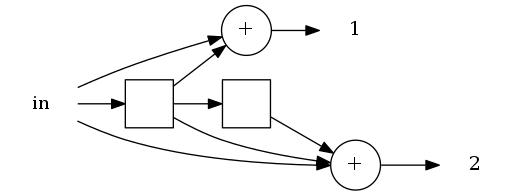
\includegraphics[scale=.5]{assets/conv}
  \caption{Encoder}
\end{figure}
\begin{itemize}
\item Bepaal de generator veelterm voor elke output.
\item Bepaal het toestandsdiagram
\item Bepaal $d_{min}$ en $d_{free}$
\item Encodeer een woord $110010$
\item Decodeer een ontvangen woord $v$ via het Viterbi algoritme: $10$ $01$ $10$ $00$
\end{itemize}

\subsubsection*{Antwoord}

\begin{itemize}
\item Generatorveeltermen:\\
  De outputs zijn achtereenvolgens (bij input $100..$): $(1,1)$, $(1,1)$, $(0,1)$
  \begin{itemize}
  \item $g^{(s)} = 1 + X$
  \item $g^{(p)} = 1 + X + X^{2}$:
  \end{itemize}
\item Toestandsdiagram:
  \begin{figure}[H]
    \centering
    \begin{tikzpicture}[->,>=stealth',shorten >=1pt,auto,node distance=3cm,
      thick,main node/.style={circle,fill=blue!20,draw,font=\sffamily\Large\bfseries}]

      \node[main node] (10) {10};
      \node[main node] (00) [below left of=10] {00};
      \node[main node] (11) [below right of=10] {11};
      \node[main node] (01) [below right of=00] {01};

      \path[every node/.style={font=\sffamily\small}]
      (00) edge [loop left] node {0/00} (00)
      edge node [left] {1/10} (10)
      (10) edge [bend left] node {0/11} (01)
      edge node {1/00} (11)
      (01) edge node [left] {0/01} (00)
      edge [bend left] node {1/10} (10) 
      (11) edge node [right] {0/10} (01)
      edge [loop right] node {1/01} (11);
    \end{tikzpicture}
  \end{figure}
\item 
  \begin{itemize}
  \item $d_{min}$\\
    $m$ is $2$, dus we zoeken het lichtste pad van lengte $3$ (naast het pad met enkel nullen).
    De lichtste paden zijn $00$ $10$ $11$ $11$ en $00$ $10$ $11$ $01$ met elk gewicht $2$.
    $d_{min}$ is dus $2$.
  \item $d_{free}$\\
    Het lichtste pad dat terug naar $00$ gaat is $00$ $10$ $11$ $01$ met gewicht $3$.
    $d_{free}$ is dus $3$.
  \end{itemize}
\item $c(110010) = $ $10$ $00$ $10$ $01$ $10$ $11$
\item $m(10$ $01$ $10$ $01$ $11$ $11)$\\
  Tabel van bogen
  \begin{itemize}
  \item end: einde van de boog
  \item start: begin van de boog
  \item o/p: output door de boog
  \item err: verschil tussen de output en het te decoderen frame
  \item $i$ path: totale afstand tot nu toe
  \item $f$ path: som van err en $i$ path
  \end{itemize}
  \begin{itemize}
  \item Start: State: $00$
    \[
    \begin{array}{ccccccc}
      \hline
      \text{end} & \text{start} & \text{o/p} & \text{err} & i \text{ path } & f \text{ path} & \text{keep}\\
      \hline
      00 & 00 & 00 & & 0 & \infty & \\
      00 & 01 & 01 & & \infty & \infty & \\
      01 & 10 & 11 & & \infty & \infty & \\
      01 & 11 & 10 & & \infty & \infty & \\
      10 & 00 & 10 & & 0 & \infty & \\
      10 & 01 & 10 & & \infty & \infty & \\
      11 & 10 & 00 & & \infty & \infty & \\
      11 & 11 & 01 & & \infty & \infty & \\
      \hline
    \end{array}
    \]
  \item Frame: $10$
    \[
    \begin{array}{ccccccc}
      \hline
      \text{end} & \text{start} & \text{o/p} & \text{err} & i \text{ path } & f \text{ path} & \text{keep}\\
      \hline
      00 & 00 & 00 & 1 & 0 & 1 & Y\\
      00 & 01 & 01 & 2 & \infty & \infty & \\
      01 & 10 & 11 & 1 & \infty & \infty & Y\\
      01 & 11 & 10 & 0 & \infty & \infty & \\
      10 & 00 & 10 & 0 & 0 & 0 & Y\\
      10 & 01 & 10 & 0 & \infty & \infty & \\
      11 & 10 & 00 & 1 & \infty & \infty & Y\\
      11 & 11 & 01 & 2 & \infty & \infty & \\
      \hline
    \end{array}
    \]
  \item Frame: $01$
    \[
    \begin{array}{ccccccc}
      \hline
      \text{end} & \text{start} & \text{o/p} & \text{err} & i \text{ path } & f \text{ path} & \text{keep}\\
      \hline
      00 & 00 & 00 & 1 & 1 & 2 & Y\\
      00 & 01 & 01 & 0 & \infty & \infty & \\
      01 & 10 & 11 & 1 & 0 & 1 & Y\\
      01 & 11 & 10 & 2 & \infty & \infty & \\
      10 & 00 & 10 & 2 & 1 & 3 & Y\\
      10 & 01 & 10 & 2 & \infty & \infty & \\
      11 & 10 & 00 & 1 & 0 & 1 & Y\\
      11 & 11 & 01 & 0 & \infty & \infty & \\
      \hline
    \end{array}
    \]
  \item Frame: $10$
    \[
    \begin{array}{ccccccc}
      \hline
      \text{end} & \text{start} & \text{o/p} & \text{err} & i \text{ path } & f \text{ path} & \text{keep}\\
      \hline
      00 & 00 & 00 & 1 & 2 & 3 & \\
      00 & 01 & 01 & 2 & 1 & 3 & Y\\
      01 & 10 & 11 & 1 & 3 & 4 & \\
      01 & 11 & 10 & 0 & 1 & 1 & Y\\
      10 & 00 & 10 & 0 & 2 & 2 & \\
      10 & 01 & 10 & 0 & 1 & 1 & Y\\
      11 & 10 & 00 & 1 & 3 & 4 & \\
      11 & 11 & 01 & 2 & 1 & 3 & Y\\
      \hline
    \end{array}
    \]
  \item Frame: $01$
    \[
    \begin{array}{ccccccc}
      \hline
      \text{end} & \text{start} & \text{o/p} & \text{err} & i \text{ path } & f \text{ path} & \text{keep}\\
      \hline
      00 & 00 & 00 & 1 & 3 & 4 & \\
      00 & 01 & 01 & 0 & 1 & 1 & Y\\
      01 & 10 & 11 & 1 & 1 & 2 & Y\\
      01 & 11 & 10 & 2 & 3 & 5 & \\
      10 & 00 & 10 & 2 & 3 & 5 & \\
      10 & 01 & 10 & 2 & 1 & 3 & Y\\
      11 & 10 & 00 & 1 & 1 & 2 & Y\\
      11 & 11 & 01 & 0 & 3 & 3 & \\
      \hline
    \end{array}
    \]
  \item Frame: $11$
    \[
    \begin{array}{ccccccc}
      \hline
      \text{end} & \text{start} & \text{o/p} & \text{err} & i \text{ path } & f \text{ path} & \text{keep}\\
      \hline
      00 & 00 & 00 & 2 & 1 & 3 & \\
      00 & 01 & 01 & 1 & 2 & 3 & Y\\
      01 & 10 & 11 & 0 & 3 & 3 & \\
      01 & 11 & 10 & 1 & 2 & 3 & Y\\
      10 & 00 & 10 & 1 & 1 & 2 & Y\\
      10 & 01 & 10 & 1 & 2 & 3 & \\
      11 & 10 & 00 & 2 & 3 & 5 & \\
      11 & 11 & 01 & 1 & 2 & 3 & Y\\
      \hline
    \end{array}
    \]
  \item Frame: $11$
    \[
    \begin{array}{ccccccc}
      \hline
      \text{end} & \text{start} & \text{o/p} & \text{err} & i \text{ path } & f \text{ path} & \text{keep}\\
      \hline
      00 & 00 & 00 & 2 & 3 & 5 & \\
      00 & 01 & 01 & 1 & 3 & 4 & Y\\
      01 & 10 & 11 & 0 & 2 & 2 & Y\\
      01 & 11 & 10 & 1 & 3 & 4 & \\
      10 & 00 & 10 & 1 & 3 & 4 & Y\\
      10 & 01 & 10 & 1 & 3 & 4 & \\
      11 & 10 & 00 & 2 & 2 & 4 & Y\\
      11 & 11 & 01 & 1 & 3 & 4 & \\
      \hline
    \end{array}
    \]
  \item We zoeken het pad terug: $00$ $10$ $11$ $01$ $00$ $10$ $01$
  \item Dit komt overeen met een informatiewoord $110010$.
  \end{itemize}
\end{itemize}






\end{document}
